\documentclass{article}
\usepackage{graphicx} % Required for inserting images
\usepackage[table,xcdraw]{xcolor}
\usepackage{colortbl} 

\title{Teste}
\author{Bertaco}
\begin{document}

\maketitle

\section*{*dado1*}

\begin{center}
    \begin{table}[h]
    \begin{tabular}{|lc|}
    \hline
    \multicolumn{2}{|c|}{\cellcolor[HTML]{002060}{\color[HTML]{FFFFFF} Informacoes   Gerais}} \\ \hline
\multicolumn{1}{|l|}{Codigo} & teste \\ \hline
    \multicolumn{1}{|l|}{Nome} & teste \\ \hline
    \multicolumn{1}{|l|}{Categoria} & teste \\ \hline
    \multicolumn{1}{|l|}{Fornecedor} & teste \\ \hline
    \multicolumn{1}{|l|}{NCM} & teste \\ \hline
    \end{tabular}
    \end{table}
\end{center}

\begin{center}
    \begin{figure}[h]
        \centering
        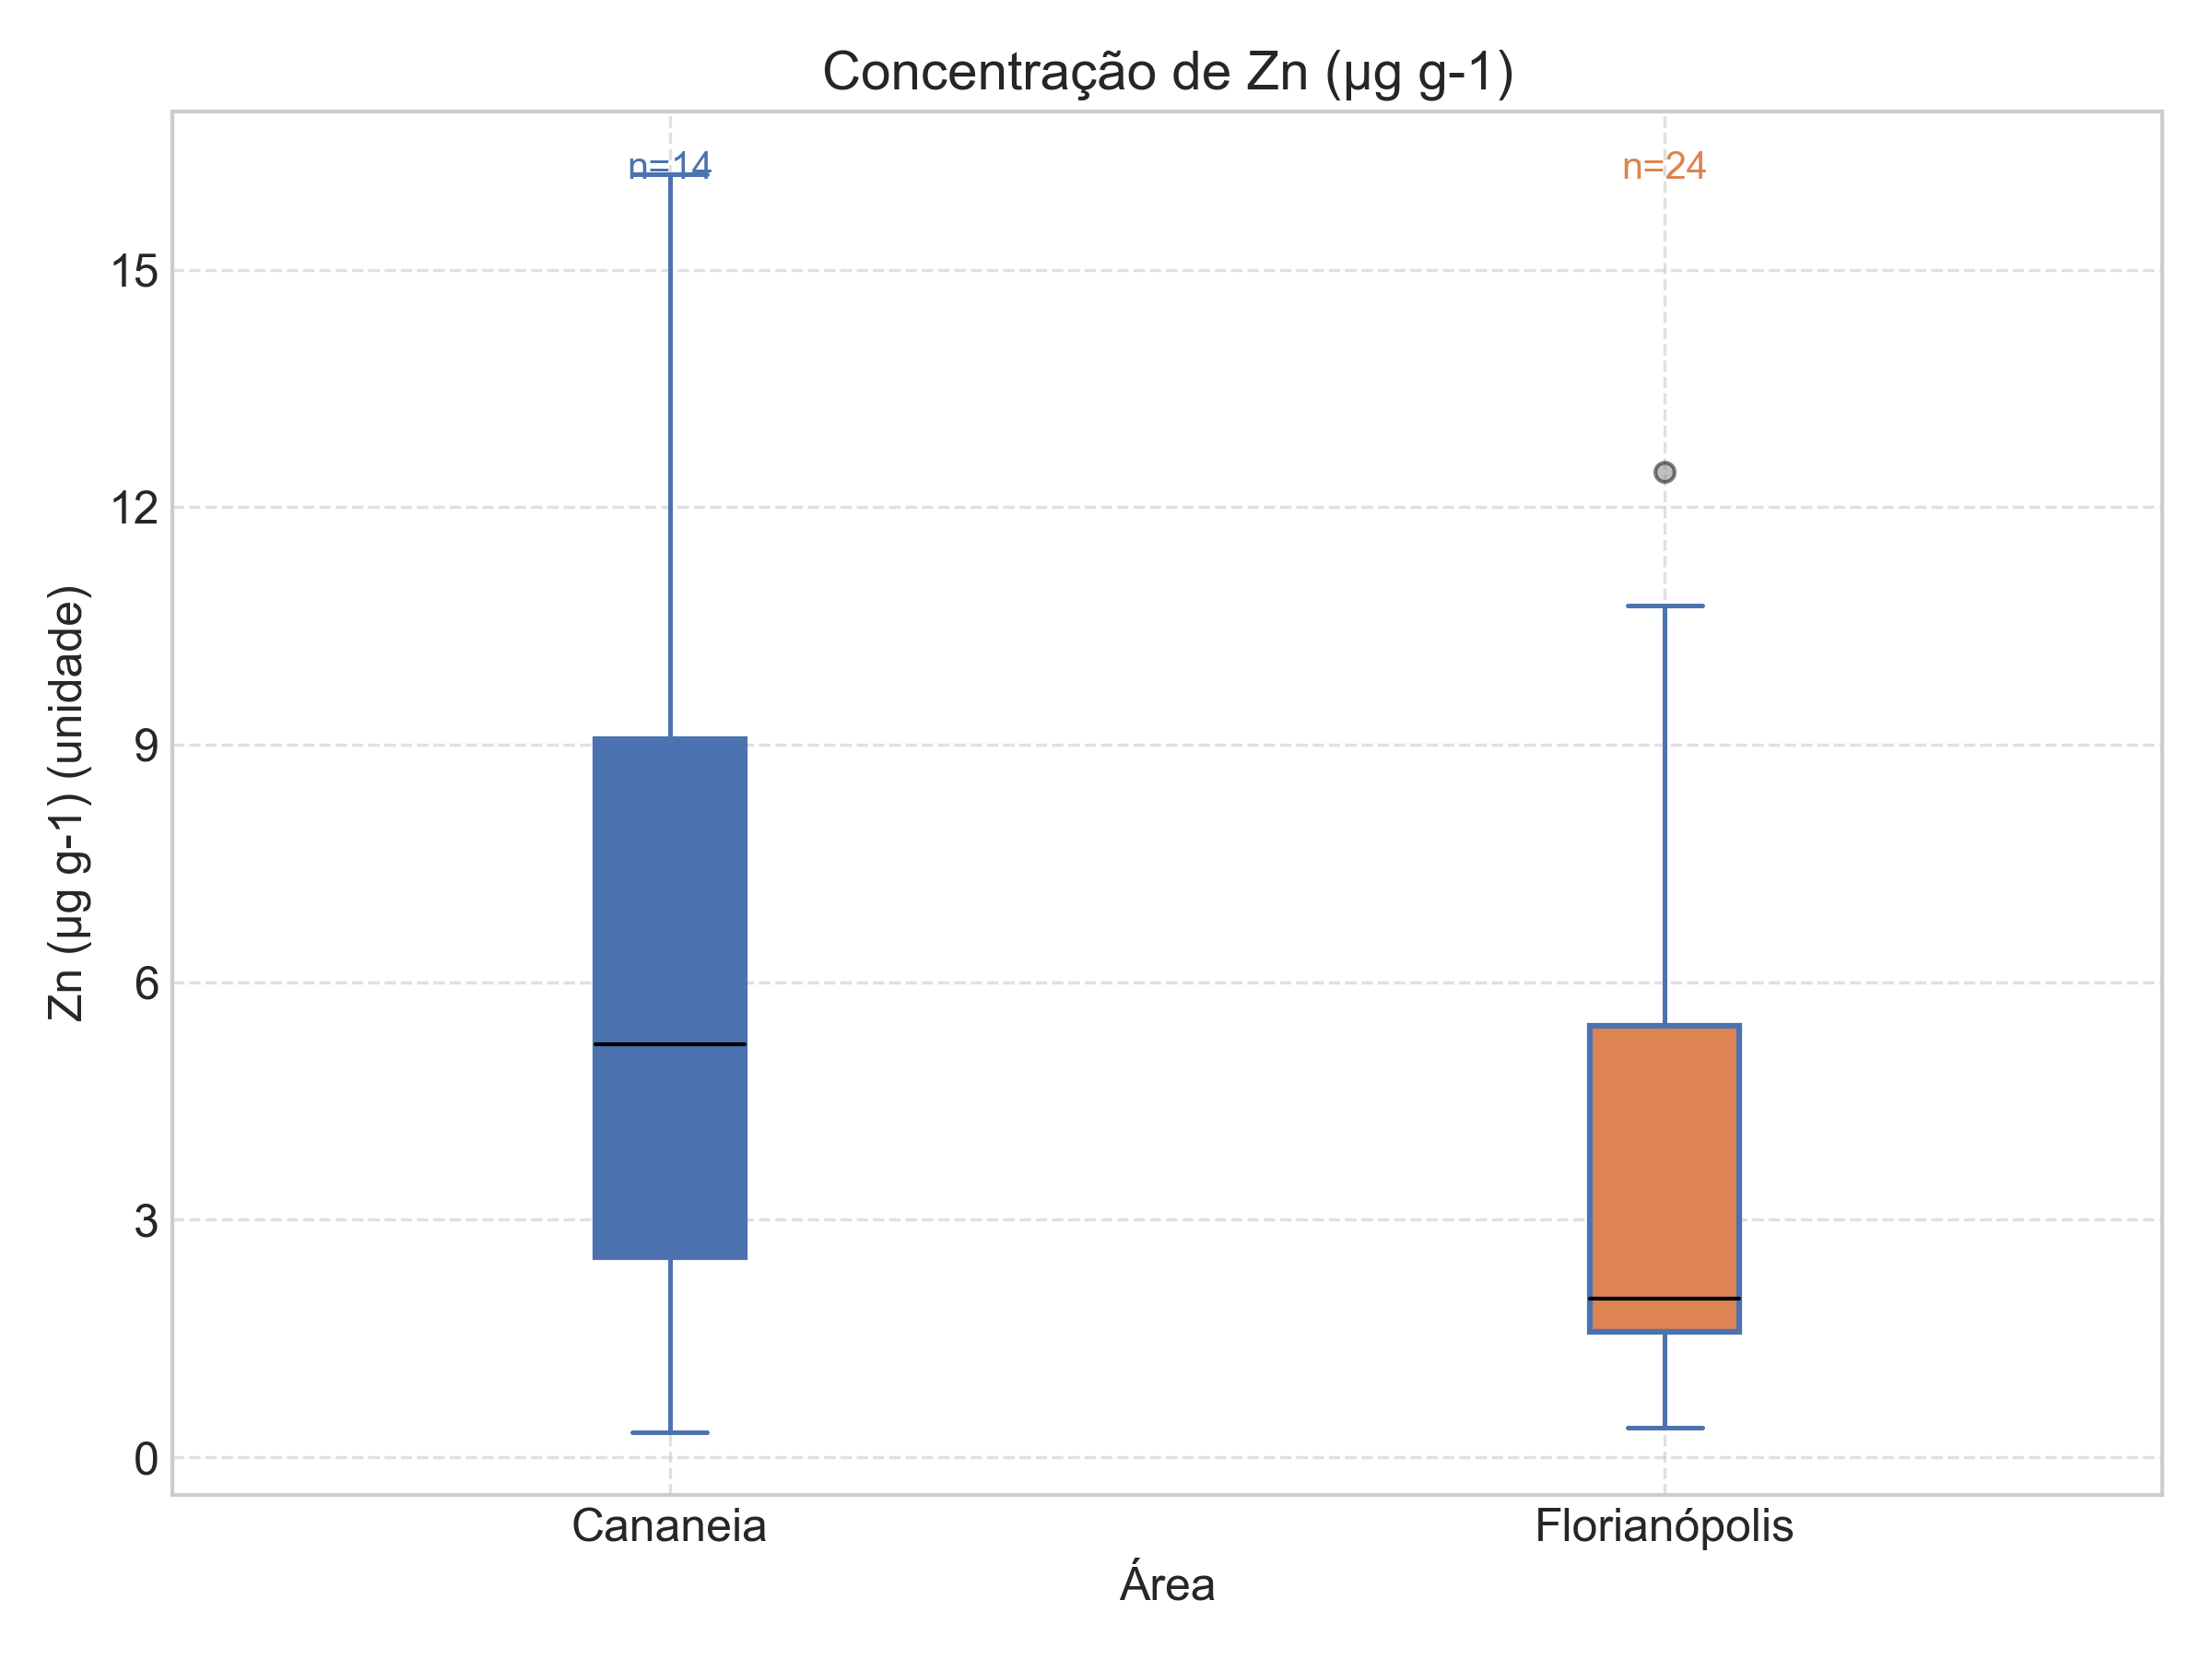
\includegraphics[width=0.7\linewidth]{imagem.png}
        \caption{Enter Caption}
        \label{fig:placeholder}
    \end{figure}
\end{center}

\section*{*dado2*}
\end{document}
